\documentclass[10pt]{beamer}
\usepackage{amsmath}
\usepackage{amssymb}
%\usepackage{dsfont}
\usepackage{accents}
\usepackage{hyphenat}
\usepackage{multirow}
\usepackage{hyperref}
\usetheme[progressbar=frametitle]{metropolis}
\usepackage{appendixnumberbeamer}
\usefonttheme[onlymath]{serif}
\usepackage{booktabs}
\usepackage[scale=2]{ccicons}
\usepackage{animate}
\usepackage{xcolor}
\usepackage{soul}

%\usepackage{pgfplots}
%\usepgfplotslibrary{dateplot}
%\usepgflibrary{arrows}

\usepackage{xspace}
\newcommand{\themename}{\textbf{\textsc{metropolis}}\xspace}
\usetikzlibrary{snakes,arrows,mindmap,trees,backgrounds,shapes.geometric}
\tikzset{graphics/.style={inner sep=0,outer sep=0}}
\tikzset{scaleall/.style={scale=#1, transform shape}}



\newlength{\bbw}
\newlength{\bbh}
\newcommand{\pcuad}[3][]{
  % First arguments is an optional prefix for the coordinate names

  \setlength{\bbw}{#2}
  \setlength{\bbh}{#3}
  \useasboundingbox(0,0) rectangle (\bbw,\bbh);

  \path(.5\bbw,.5\bbh) coordinate(#1cp);
  \path(\bbw,0)        coordinate(#1se);
  \path(0,0)           coordinate(#1sw);
  \path(0,\bbh)        coordinate(#1nw);
  \path(\bbw,\bbh)     coordinate(#1ne);
 
  
  \path(\bbw,.5\bbh) coordinate(#1ep);
  \path(.5\bbw,0)    coordinate(#1sp);
  \path(.5\bbw,\bbh) coordinate(#1np);
  \path(0,.5\bbh)    coordinate(#1wp);
       
  \path(.75\bbw,.5\bbh) coordinate(#1hr);
  \path(.25\bbw,.5\bbh) coordinate(#1hl);
  \path(.5\bbw,.25\bbh) coordinate(#1vl);
  \path(.5\bbw,.75\bbh) coordinate(#1vu);

  \path(.75\bbw,.75\bbh) coordinate(#1c1);
  \path(.25\bbw,.75\bbh) coordinate(#1c2);
  \path(.25\bbw,.25\bbh) coordinate(#1c3);
  \path(.75\bbw,.25\bbh) coordinate(#1c4);


%  +-----------------------------------------------+
%  |nw                    np                     ne|
%  |                                               |
%  |                                               |
%  |          c2          vu          c1           |
%  |                                               |
%  |                                               |
%  |wp        hl          cp          hr         ep|
%  |                                               |
%  |                                               |
%  |          c3          vl          c4           |
%  |                                               |
%  |                                               |
%  |sw                    sp                     se|
%  +-----------------------------------------------+
}
 
        
\newcommand{\showcuad}[1][]{

   \draw[help lines,xstep=.5,ystep=.5,gray!10] (#1sw) grid (#1ne);
   \draw[help lines,xstep=1,ystep=1,gray]      (#1sw) grid (#1ne);
   %\draw[help lines,xstep=.25,ystep=.25,gray!20] (sw) grid (ne);
   % \draw[help lines,xstep=1,ystep=1,gray] (sw) grid (ne);
   % \foreach \x in {-20,-14.5,...,20} {
   %     \node [anchor=north, gray,yshift=30] at (\x,0) {\tiny \bf \x};
   %     \node [anchor=east,gray,xshift=30] at (0,\x) {\tiny \bf  \x};
   % }
               
    \fill(#1se) circle(.1) node[anchor=south east]{#1se};
    \fill(#1sw) circle(.1) node[anchor=south west]{#1sw};
    \fill(#1ne) circle(.1) node[anchor=north east]{#1ne};
    \fill(#1nw) circle(.1) node[anchor=north west]{#1nw};
                  
    \fill(#1hr) circle(.1) node[above]{#1hr};
    \fill(#1hl) circle(.1) node[above]{#1hl};
    \fill(#1vu) circle(.1) node[above]{#1vu};
    \fill(#1vl) circle(.1) node[above]{#1vl};
                  
    \fill(#1sp) circle(.1) node[anchor=south]{#1sp};
    \fill(#1wp) circle(.1) node[anchor=west] {#1wp};
    \fill(#1np) circle(.1) node[anchor=north]{#1np};
    \fill(#1ep) circle(.1) node[anchor=east] {#1ep};

    \fill(#1cp) circle(.1) node[above]{#1cp};
    \fill(#1c1) circle(.1) node[above]{#1c1};
    \fill(#1c2) circle(.1) node[above]{#1c2};
    \fill(#1c3) circle(.1) node[above]{#1c3}; 
    \fill(#1c4) circle(.1) node[above]{#1c4};

    %\fill[red](cp|-c1) circle(.1) node[anchor=north]{cp|-c1};

}

\newcommand{\ds}{\displaystyle}
\newcommand{\dsum}{\displaystyle \sum}
\newcommand{\uu}[1]{{\boldsymbol #1}}
\newcommand{\ud}{\,\mathrm{d}}
\def\ttau{\uu{\tau}}
\def\bb{\uu{b}}
\def\nb{\uu{n}}
\def\pb{\uu{p}}
\def\wb{\uu{w}}
\def\xb{\uu{x}}
\def\ab{\uu{a}}
\def\yb{\uu{y}}
\def\vb{\uu{v}}
\def\fb{\uu{f}}
\def\zb{\uu{z}}
\def\Xb{\uu{X}}
\def\etab{\uu{\eta}}
\def\thetab{\uu{\theta}}
\def\lambdab{\uu{\lambda}}
\def\gammab{\uu{\gamma}}
\def\taub{\uu{\tau}}
\def\varphib{\uu{\varphi}}
\def\Ab{\uu{A}}
\def\Bb{\uu{B}}
\def\Gb{\uu{G}}
\def\Fb{\uu{F}}
\def\Jb{\uu{J}}
\def\Rb{\uu{R}}
\def\Tb{\uu{T}}
\def\rb{\uu{r}}
\def\ab{\uu{a}}
\newcommand{\molar}[1]{\underaccent{\bar}{#1}}
\def\um{\molar{U}}
\def\hm{\molar{H}}
\def\sm{\molar{S}}
\def\am{\molar{A}}
\def\gm{\molar{G}}
\def\hh{\hat{H}}
\def\sh{\hat{S}}
\def\vm{\molar{V}}
\def\cp{C_{\rm P}}
\def\cv{C_{\rm V}}
\def\cps{C_{\rm P}^*}
\def\cvs{C_{\rm V}^*}
\def\wsd{\dot{W}_s}
\def\md{\dot{M}}\newcommand{\pd}[2]{\left(\frac{\partial {#1}}{\partial 
{#2}}\right)}
\newcommand{\tpd}[3]{\left(\frac{\partial {#1}}{\partial {#2}}\right)_{#3}}
\newcommand{\tpdn}[4]{\left(\frac{\partial^{#4} {#1}}{\partial 
{#2}^{#4}}\right)_{#3}}



\title{An introduction to modern molecular simulation methods in the biosciences}
\date{January 16, 2024}
\author{Cameron F. Abrams, \href{mailto:cfa22@drexel.edu}{cfa22@drexel.edu}\\
Bartlett '81 -- Barry '81 Professor and Head }
\institute{Department of Chemical and Biological Engineering}
\titlegraphic{\hfill
\includegraphics[height=0.75cm]{drexel-horz-blue.png}}

\begin{document}

\maketitle

\section{Introduction}

\begin{frame}[fragile]{Atoms, atoms everywhere...}

    ``If, in some cataclysm, all of scientific knowledge were to be destroyed, and only one sentence passed on to the next generations of creatures, what statement would contain the most information in the fewest words? I believe it is the atomic hypothesis … that all things are made of atoms — little particles that move around in perpetual motion, attracting each other when they are a little distance apart, but repelling upon being squeezed into one another. In that one sentence, you will see, there is an {\em enormous} amount of information about the world, if just a little \ul{imagination and thinking} are applied.''\\
    -- R. Feynman


\end{frame}


\tikzstyle{label} = [rectangle, rounded corners, minimum width=1cm, minimum height=0.5cm,text centered, draw=black, fill=red!30]
\begin{frame}{Macrostates and Microstates}
\begin{tikzpicture}[scaleall=1.0,node distance=3cm]]
\node (pic) [] {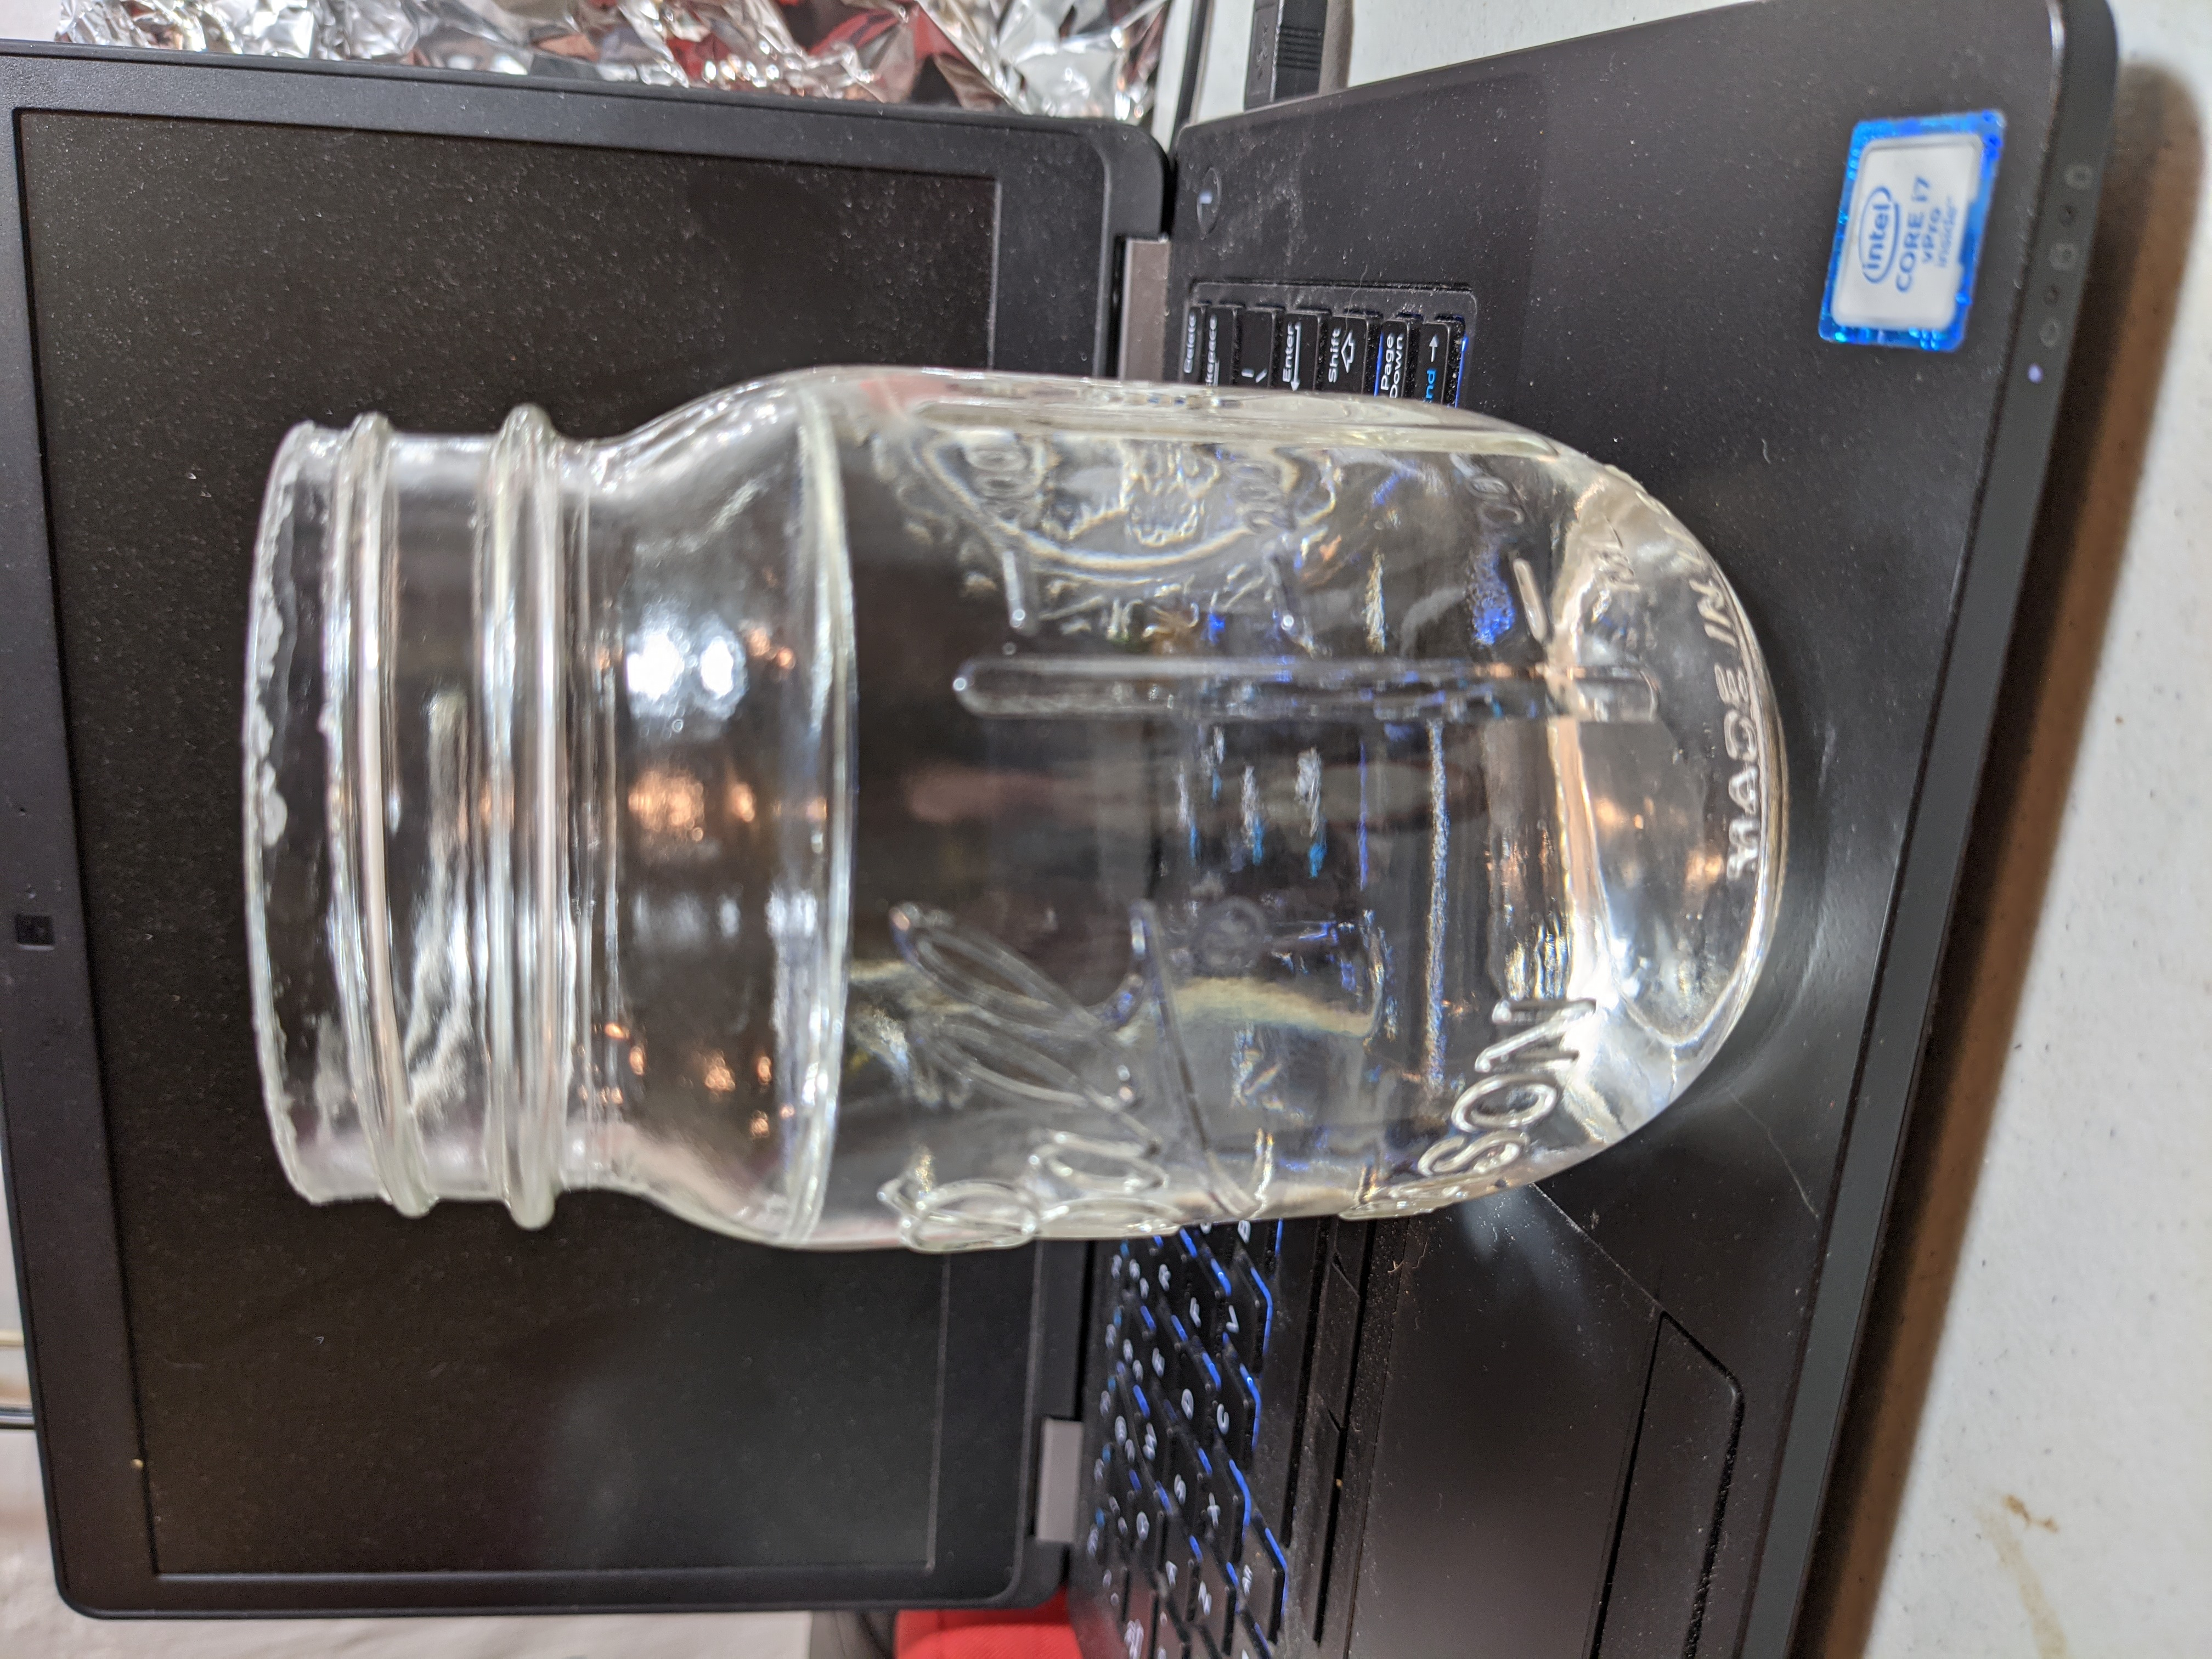
\includegraphics[angle=270,width=0.4\textwidth]{water-pic.jpg}};
\node (label1) [label,below of=pic,yshift=-1cm] {Macrostate}; 
\node (graphic1) [right of=pic,xshift=3cm,yshift=-0.1cm] {
        \animategraphics[loop,controls,width=0.5\textwidth]{10}{movie-water-md/water.000}{00}{90}
    };
\node (label2) [label,below of=graphic1,yshift=-0.9cm] {Microstates (MD)}; 
\end{tikzpicture}
\end{frame}

\section{Molecular Dynamics}

\tikzstyle{startstop} = [rectangle, rounded corners, minimum width=1cm, minimum height=0.5cm,text centered, draw=black, fill=red!30]
\tikzstyle{io} = [trapezium, trapezium left angle=70, trapezium right angle=110, minimum width=1cm, minimum height=0.5cm, text centered, draw=black, fill=blue!30]
\tikzstyle{process} = [rectangle, minimum width=1cm, minimum height=1cm, text centered, draw=black, fill=orange!30]
\tikzstyle{decision} = [diamond, minimum width=1cm, minimum height=1cm, text centered, draw=black, fill=green!30]
\tikzstyle{myarrow} = [thick,->,>=stealth]
\begin{frame}[fragile]{Molecular Dynamics (MD)}
\begin{tikzpicture}[scaleall=1.0,node distance=2cm]
\node (start) [startstop] {Start};
\node (init) [io,right of=start,xshift=1cm,text width=2cm] {Initial atomic positions and velocities};
\node (force) [process,right of=init,xshift=1cm] {Get forces};
\node (integrate) [process,below of=force] {Update positions and velocities};
\node (check) [decision,below of=integrate] {Done?};
\node (continue) [process,right of=check,xshift=1cm] {\begin{tabular}{c} Update time \\ by 10$^{-15}$ s \end{tabular}};
\node (terminate) [process,left of=check,xshift=-1cm] {Save data};
\node (stop) [startstop,left of=terminate] {Stop};
\draw [myarrow] (start) -- (init);
\draw [myarrow] (init) -- (force);
\draw [myarrow] (force) -- (integrate);
\draw [myarrow] (integrate) -- (check);
\draw [myarrow] (check) -- node[anchor=south] {no} (continue);
\draw [myarrow] (continue) |- (force);
\draw [myarrow] (check) -- node[anchor=south] {yes} (terminate);
\draw [myarrow] (terminate) -- (stop);
\end{tikzpicture}
\end{frame}


\begin{frame}[fragile]{Lengthening the Reach of Molecular Dynamics Simulations}
%\vspace{5mm}
%\hspace{-5mm}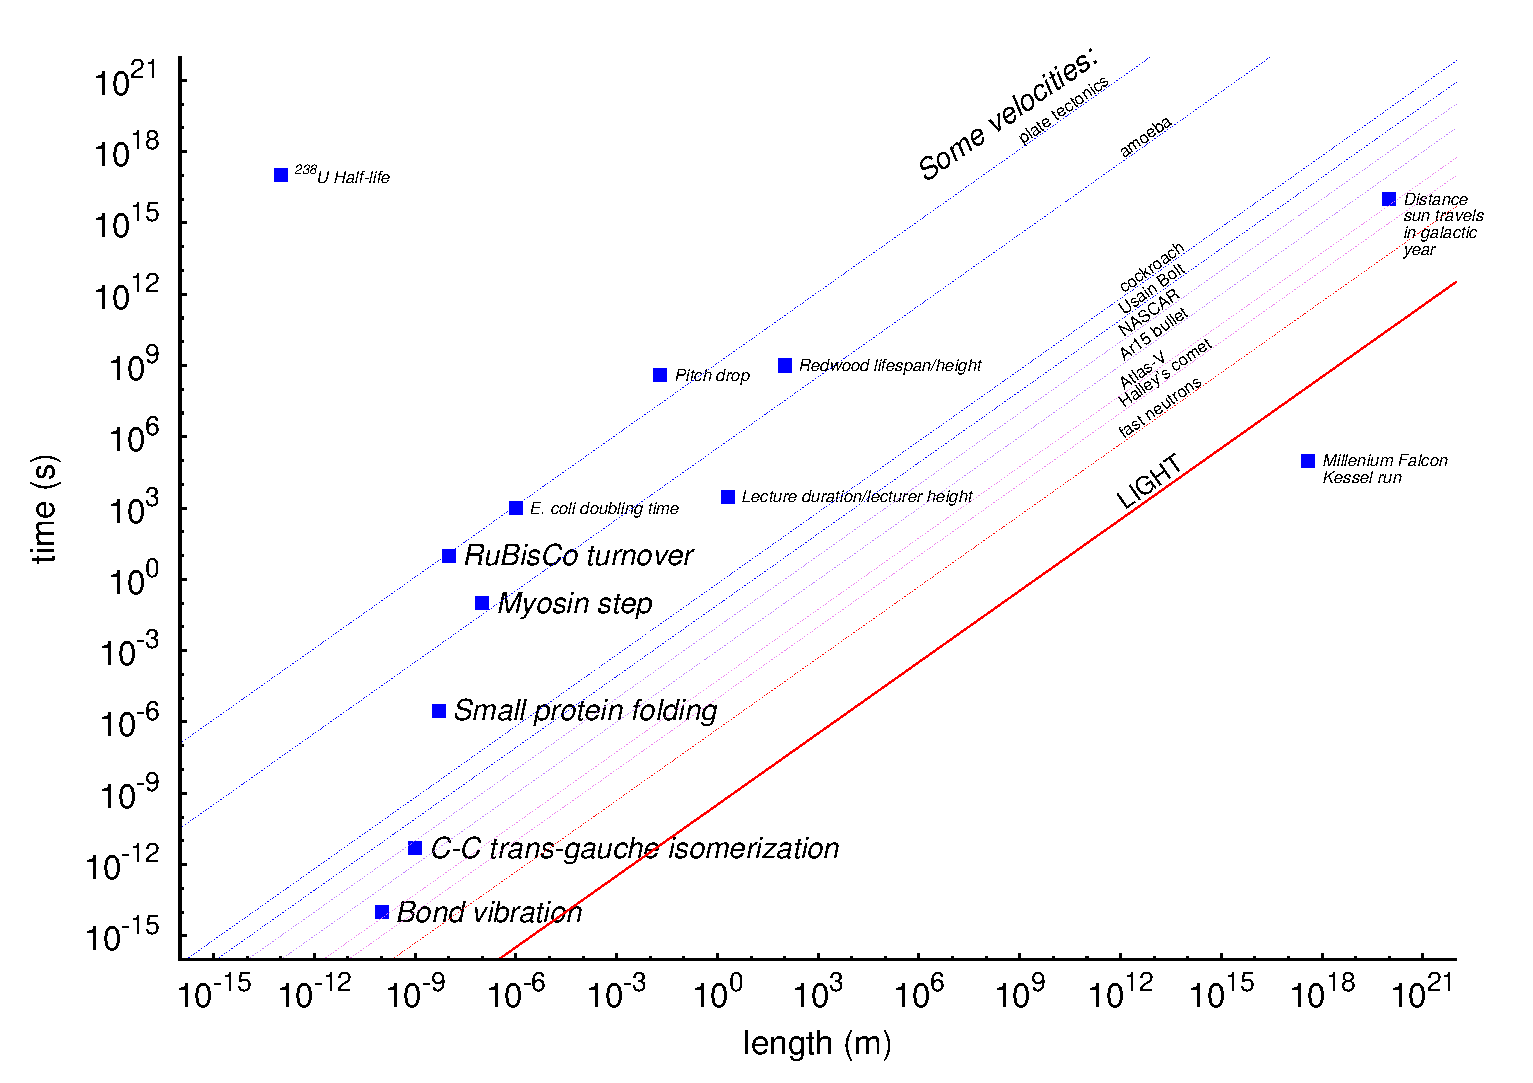
\includegraphics[width=\textwidth]{time_vs_length.eps}
\begin{tikzpicture}[scale=1.5]
\node[anchor=south west,inner sep=0] (image) at (0,0) 
{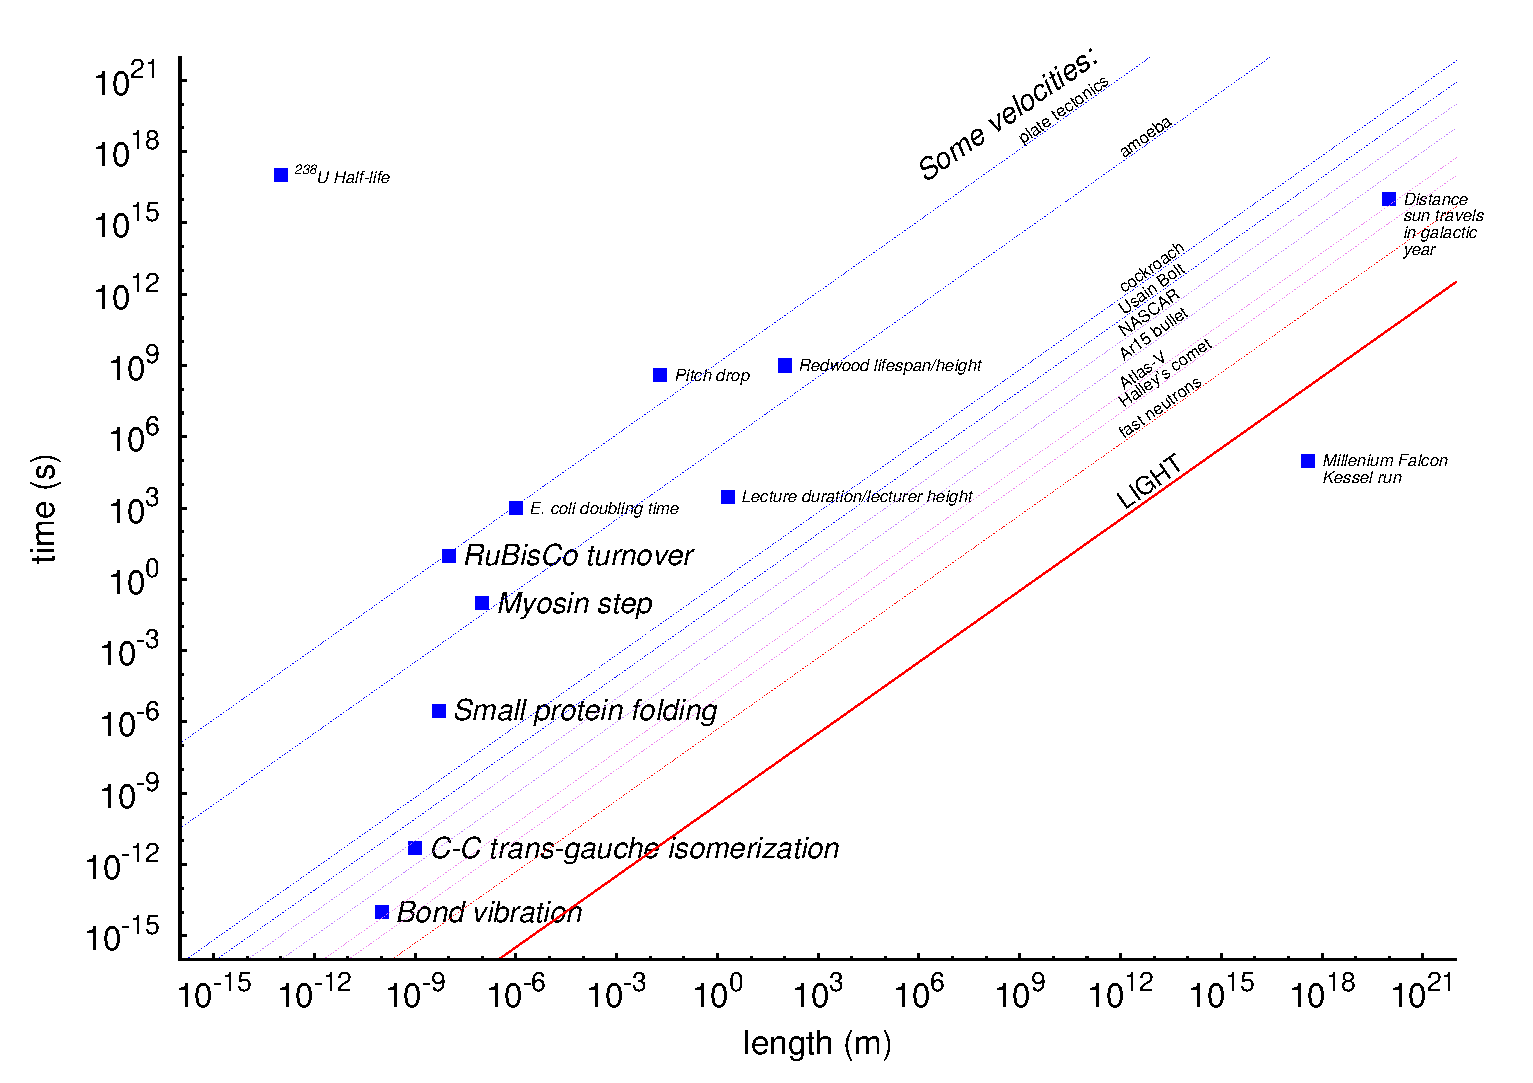
\includegraphics[width=0.975\textwidth]{time_vs_length.eps}};
\begin{scope}[x={(image.south east)},y={(image.north west)}]
\draw[red,thick,rounded corners] (0.2,0.125) rectangle (0.32,0.375);
\draw[red,thick] (0.26,0.275) node {MD};
\draw[->, green!80!black, thick, snake=snake, segment amplitude=.4mm, segment length=2mm, 
line after snake=1mm] (0.29,0.375) -- (0.29,0.45);
\draw[->, green!80!black, thick, snake=snake, segment amplitude=.4mm, segment length=2mm, 
line after snake=1mm] (0.26,0.375) -- (0.26,0.475);
\draw[->, green!80!black, thick, snake=snake, segment amplitude=.4mm, segment length=2mm, 
line after snake=1mm] (0.23,0.375) -- (0.23,0.5);
\draw[->, blue!80!white, thick, snake=snake, segment amplitude=.4mm, segment length=2mm, 
line after snake=1mm] (0.32,0.285) -- (0.38,0.285);
\draw[->, blue!80!white, thick, snake=snake, segment amplitude=.4mm, segment length=2mm, 
line after snake=1mm] (0.32,0.25) -- (0.4,0.25);
\node[green!80!black,text width=2cm,rotate=90] at (0.25,0.65) {Enhanced sampling};
%\draw [red,thick,rotate=-90] (0.3,0.6) node {Enhanced Sampling};
\draw [blue!80!white,thick] (0.57,0.27) node {Resolution coarsening};
\end{scope}
\end{tikzpicture}
\end{frame}



\begin{frame}{The Essential Problem: Poor Sampling of Feature Space}
\begin{tikzpicture}[scaleall=1.0]
\pcuad{\textwidth}{\textheight}
\path(nw) ++(-1,-0.5) node(graphic1)[anchor=north west]{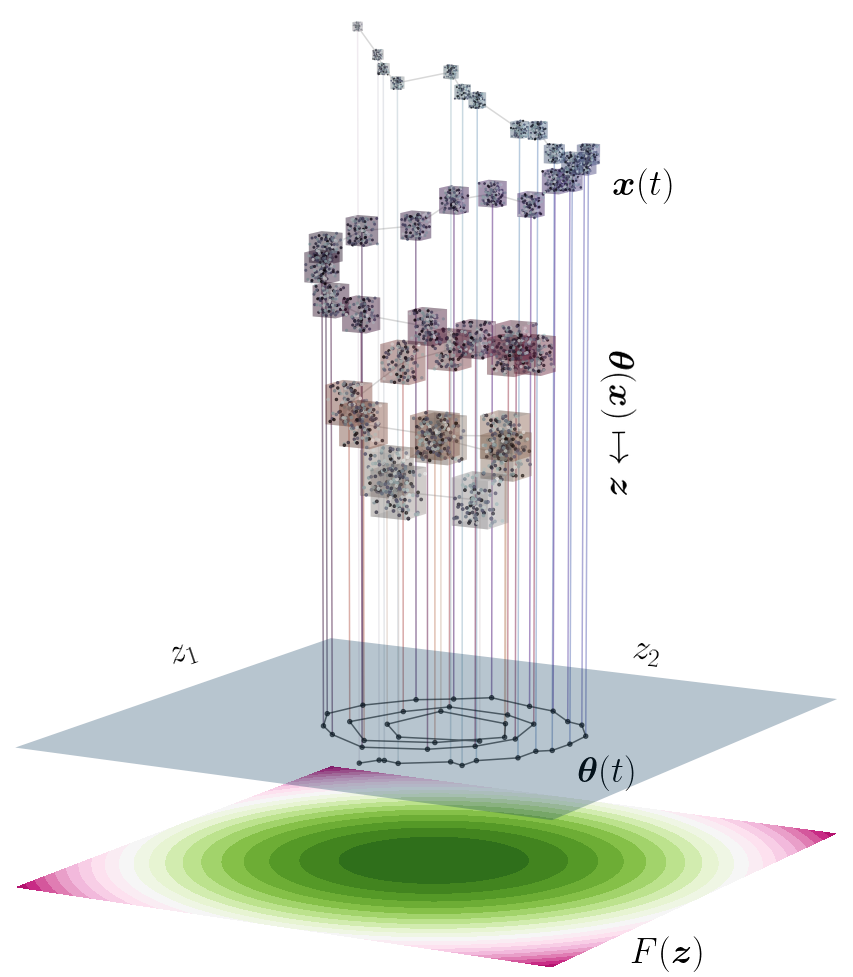
\includegraphics[width=0.6\textwidth]{hmmdfig-crop.png}};
\path(np) ++(-1,0) node(line1)[anchor=north west]{Configuration space $\xb^{3N} \equiv [(x_0,x_1,x_2)_1,\dots]$}
          ++(0,-1) node(line2)[anchor=west]{MD: $m_i\ddot{x}_i = -\nabla_iV(\xb) + \mbox{ensemble forces}$}
          ++(1,-1) node(line3)[anchor=west]{Samples $\Rightarrow\ \xb(t_1),\ \xb(t_2),\ \dots$}
          ++(0,-1) node(line4)[anchor=west]{Ergodicity: $\displaystyle\langle X\rangle \approx \frac{1}{n_\tau}\sum_{i=1}^{n_\tau} X[\xb(t_i)]$}
          ++(-1.3,-1) node(line5)[anchor=west]{Mapping configuration space}
          ++(0,-0.4) node(line5)[anchor=west]{to feature space}
          ++(0.25,-1.) node(line6)[anchor=west]{Feature space: $\zb^M \equiv (z_1,z_2,\dots)$}
          ++(0,-2) node(line7)[anchor=west]{Free energy: $F(\zb)=-k_{\rm B}T\ln\langle\delta\left[\theta(\xb)-\zb\right]\rangle$};
\end{tikzpicture}
\end{frame}


\section{Computational Drug Design}

\section{Summary}

\begin{frame}[fragile]{Summary}
\begin{itemize}
\item \textcolor{red}{OTFP} combines enhanced sampling and free-energy-profile generation to provide deeper understanding of biomolecular mechanisms
\begin{itemize}
\item We rationalized DAVEI activity dependence on linker length
\item We recapitulate water-mediated ``knock-on'' transport of multiple K$^+$ ions in Kv1.2, but also predict reduced barriers for dry transport
\end{itemize}
\item Demonstrated the \textcolor{magenta!80!black}{Climbing Multistrings Method} for locating stationary points in feature space
\item Demonstrated \textcolor{green!80!black}{Markovian milestoning} along minimum free-energy pathways to estimate entry and exit rates of O$_{\sf 2}$ in MSOX
\begin{itemize}
\item MSOX: Simulations agree with experiment that modified ping-pong mechanism is more likely than ping-pong because substrate influences O$_{\sf 2}$
entry and exit kinetics
%\item MSOX: Substrate-induced gatekeeper closing and active-site desolvation likely underly the substrates effect on O$_{\sf 2}$.
\end{itemize}
\end{itemize}
\end{frame}

% \begin{frame}[fragile]{Acknowledgments}
\begin{tikzpicture}[scaleall=1.0]
\pcuad{\textwidth}{\textheight}
%\showcuad
\path(nw) ++(-0.5,0.0) node(text1) [anchor=north west,text width=1.1\textwidth,execute at begin node=\setlength{\baselineskip}{1em}]{
\begin{itemize}
\item {\bf OTFP:}  \textcolor{red!80!black}{Dr. S. Alexis PAZ} (N. U. C\'ordoba, Argentina) and Dr. Steven GOSSERT (2021)
\item {\bf Climbing Multistrings:} \textcolor{green!80!black}{Dr. Gourav SHRIVASTAV}
\item {\bf Milestoning:} {\small \textcolor{blue!80!black}{Dr. Anthony BUCCI} (West Pharma)}
\item {\bf Other current projects:}
\begin{itemize}
\item Natasha VERGARA (2022):  HIV-1 Entry Inhibitor Design
\item Ming HUANG (2022):  Molecular modeling of thermosets
\item Dr. Salman ZARRINI:  Molecular modeling of thermoset/glass sizing fluid
\item Dr. Mohammadjavad MOHAMMADI:  HIV-1 Entry Inhibitor Design
\end{itemize}
\item {\bf Collaborators}
\begin{itemize}
\item \textcolor{magenta!80!black}{Prof. Eric VANDEN-EIJNDEN} (NYU; Mathematics)
\item Prof. Irwin CHAIKEN (DUCOM; Biochemistry)
\item Prof. Amos SMITH III (UPenn; Organic Chemistry)
\end{itemize}
\end{itemize}
\begin{itemize}
\item {\bf Funding (this talk):} {\small NIH R01GM100472, NIH R01GM115249, NSF DMR1207389}
\item {\bf Resources:} {\tt www.github.com/cameronabrams/cfacv}, {\tt www.github.com/cameronabrams/psfgen}, {\tt www.github.com/cameronabrams/otfp}
\end{itemize}
};
\end{tikzpicture}
\end{frame}
  

\end{document}
